%!TeX program = xelatex
\documentclass[12pt,hyperref,a4paper,UTF8]{ctexart}
\usepackage{HDUReport}
\usepackage{listings}
\usepackage{xcolor}
\usepackage{graphicx}
\usepackage{setspace}
\usepackage{float}
\setstretch{1.5} % 设置全局行距为1.5倍

\usepackage{enumitem} % 载入enumitem包以便自定义列表环境
\setlist[itemize]{itemsep=0pt, parsep=0pt} % 设置itemize环境的项目间距和段落间距

\setmainfont{Times New Roman} % 英文正文为Times New Roman

%封面页设置
{   
    %标题
    \title{ 
        \vspace{1cm}
        \heiti \Huge \textbf{电子信息虚拟仿真实验报告} \par
        \vspace{1cm} 
        \heiti \Large {\underline{忆阻器实验2:忆阻器AC响应}   } 
        \vspace{3cm}
    
    }

    \author{
        \vspace{0.5cm}
        \kaishu\Large 学院\ \dlmu[9cm]{卓越学院} \\ %学院
        \vspace{0.5cm}
        \kaishu\Large 学号\ \dlmu[9cm]{23040447} \\ %班级
        \vspace{0.5cm}
        \kaishu\Large 姓名\ \dlmu[9cm]{陈文轩} \qquad  \\ %学号
        \vspace{0.5cm}
        \kaishu\Large 专业\ \dlmu[9cm]{智能硬件与系统(电子信息工程)} \qquad \\ %姓名 
    }
        
    \date{\today} % 默认为今天的日期,可以注释掉不显示日期
}
%%------------------------document环境开始------------------------%%
\begin{document}

%%-----------------------封面--------------------%%
\cover
\thispagestyle{empty} % 首页不显示页码
%%------------------摘要-------------%%
%\newpage
%\begin{abstract}




%\end{abstract}

%\thispagestyle{empty} % 首页不显示页码

%%--------------------------目录页------------------------%%
% \newpage
% \tableofcontents
% \thispagestyle{empty} % 目录不显示页码

%%------------------------正文页从这里开始-------------------%
\newpage
\setcounter{page}{1} % 让页码从正文开始编号

%%可选择这里也放一个标题
%\begin{center}
%    \title{ \Huge \textbf{{标题}}}
%\end{center}

\section{实验记录}

\begin{table}[H]
    \centering
    \caption{斜率法数据表}
    \begin{tabular}{|c|c|c|c|c|}
    \hline
    \textbf{频率 (Hz)} & \textbf{1} & \textbf{10} & \textbf{100} & \textbf{1000} \\ \hline
    \textbf{Gmin} &12.3 &11.42 &16 &16 \\ \hline
    \textbf{Gmax} &80&88&74.3 &93.3\\ \hline
    \end{tabular}
    \label{tab:slope_method}
\end{table}

\begin{table}[H]
    \centering
    \caption{直接读数法数据表}
    \begin{tabular}{|c|c|c|c|c|}
    \hline
    \textbf{频率 (Hz)} & \textbf{1} & \textbf{10} & \textbf{100} & \textbf{1000} \\ \hline
    \textbf{Gmin} &15&10&16& 10\\ \hline
    \textbf{Gmax} &130&110 &60&70 \\ \hline
    \end{tabular}
    \label{tab:direct_reading_method}
\end{table}


\section{上传远程平台截图}


\begin{figure}[H]
    \centering
    \begin{minipage}{1\textwidth}
        \centering
        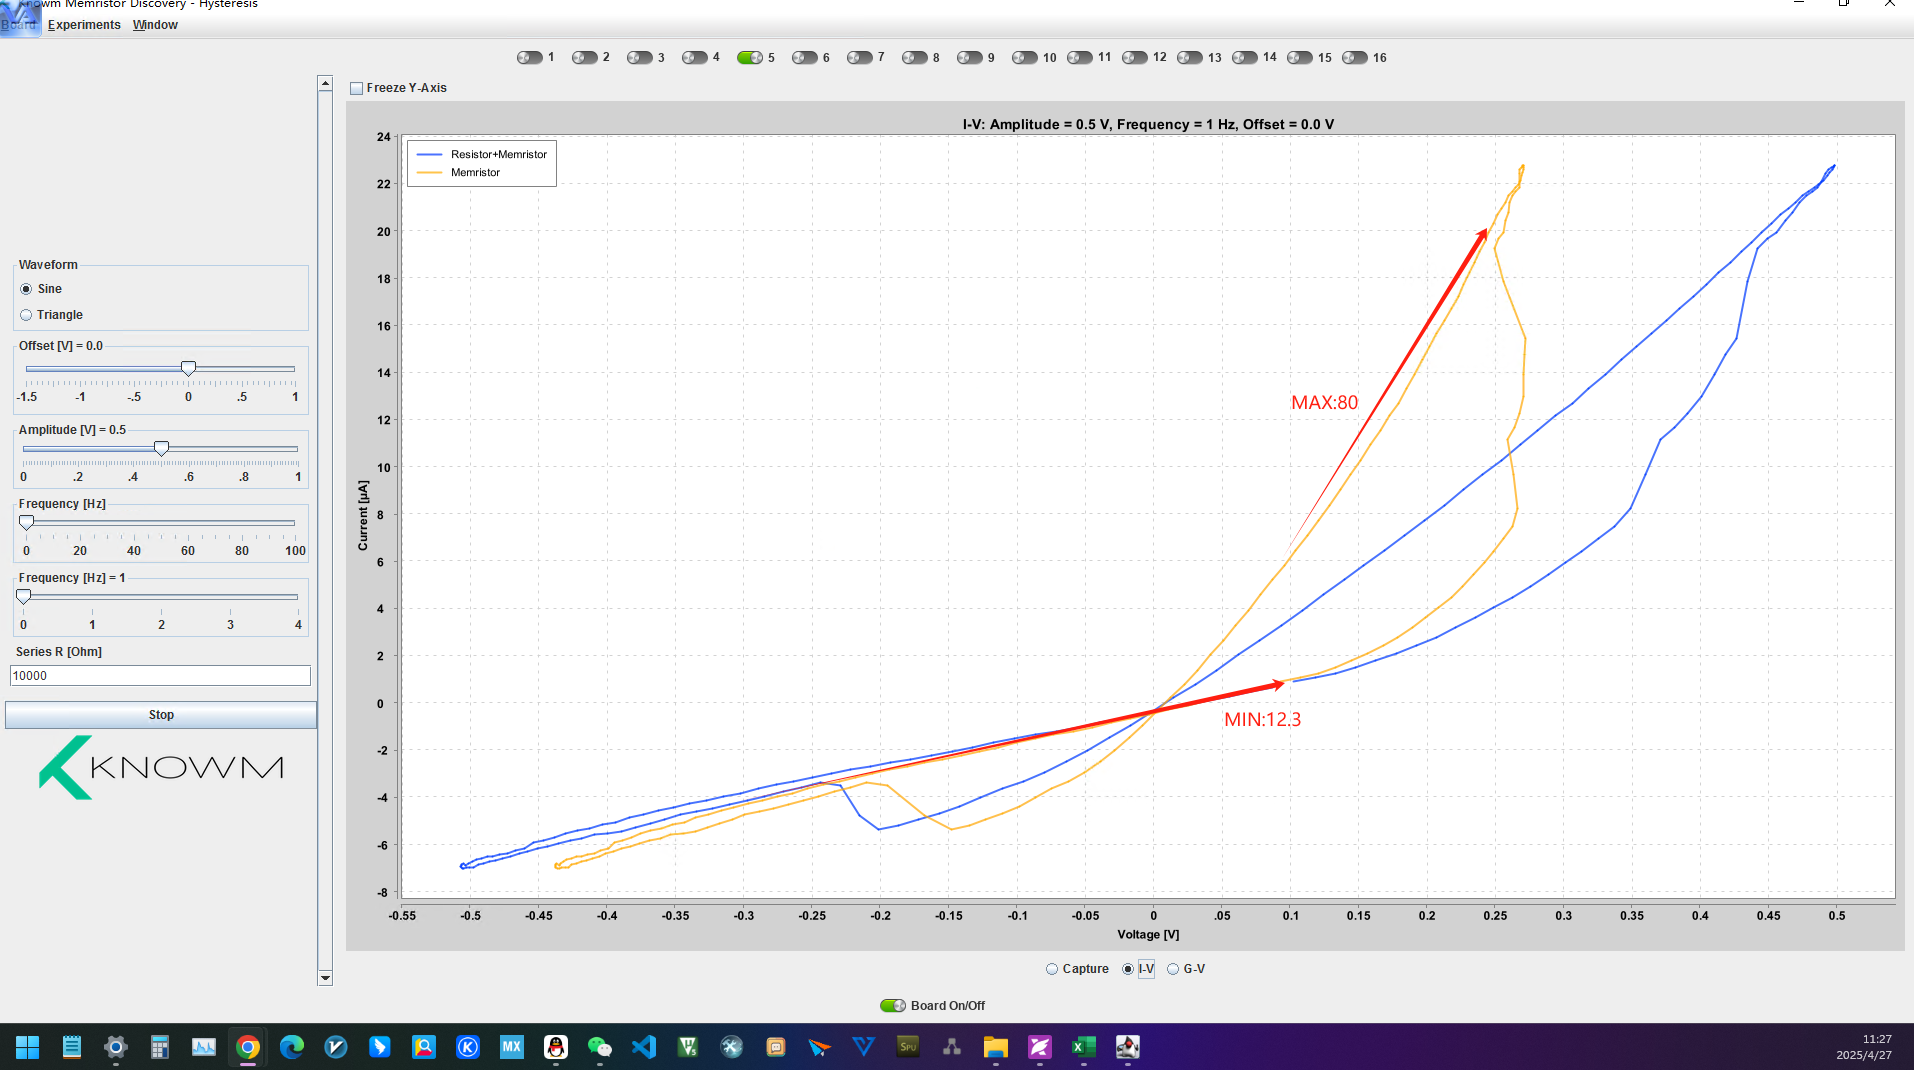
\includegraphics[width=1\textwidth]{figures/F11D.png}
        \caption{F=1,斜率法测量}
        \label{fig:system_block_diagram}
    \end{minipage}
\end{figure}


\begin{figure}[H]
    \centering
    \begin{minipage}{1\textwidth}
        \centering
        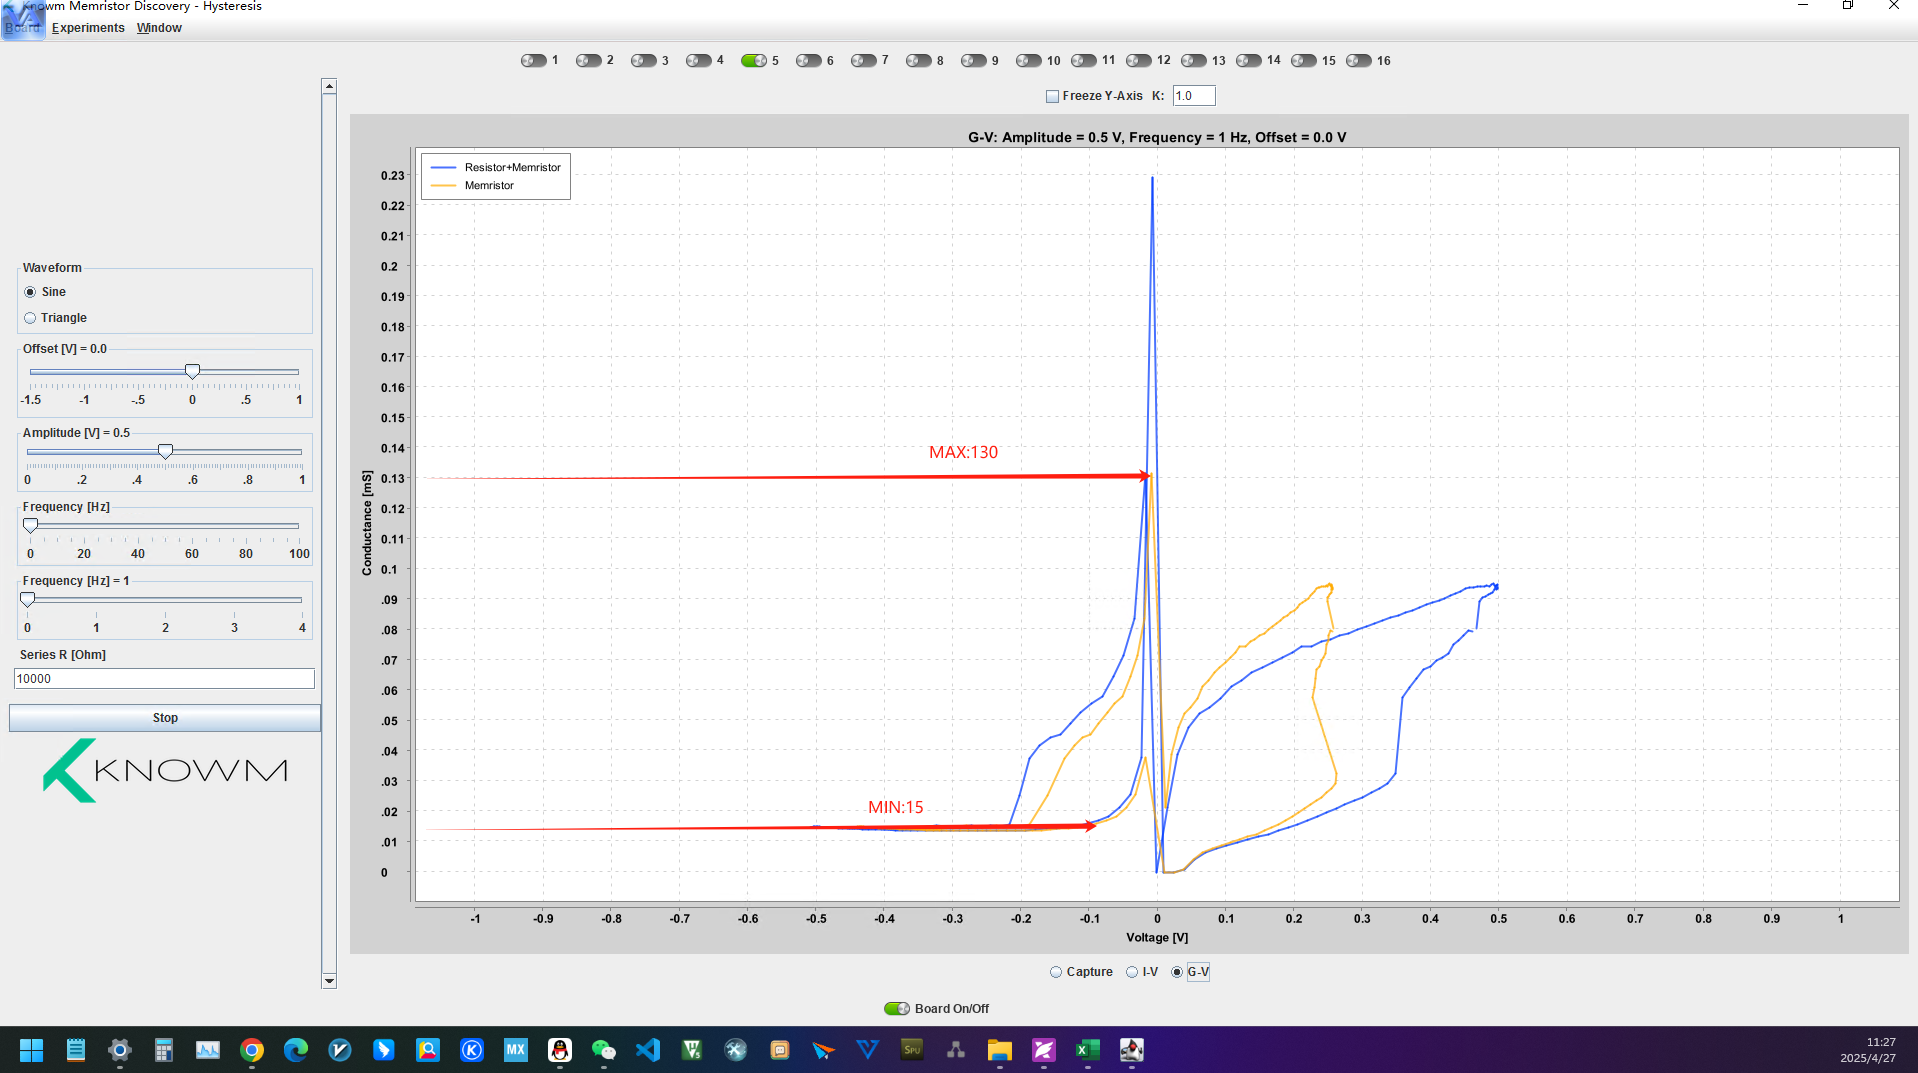
\includegraphics[width=1\textwidth]{figures/F12D.png}
        \caption{F=1,G-V直接读数法测量}
        \label{fig:system_block_diagram}
    \end{minipage}
\end{figure}

\begin{figure}[H]
    \centering
    \begin{minipage}{1\textwidth}
        \centering
        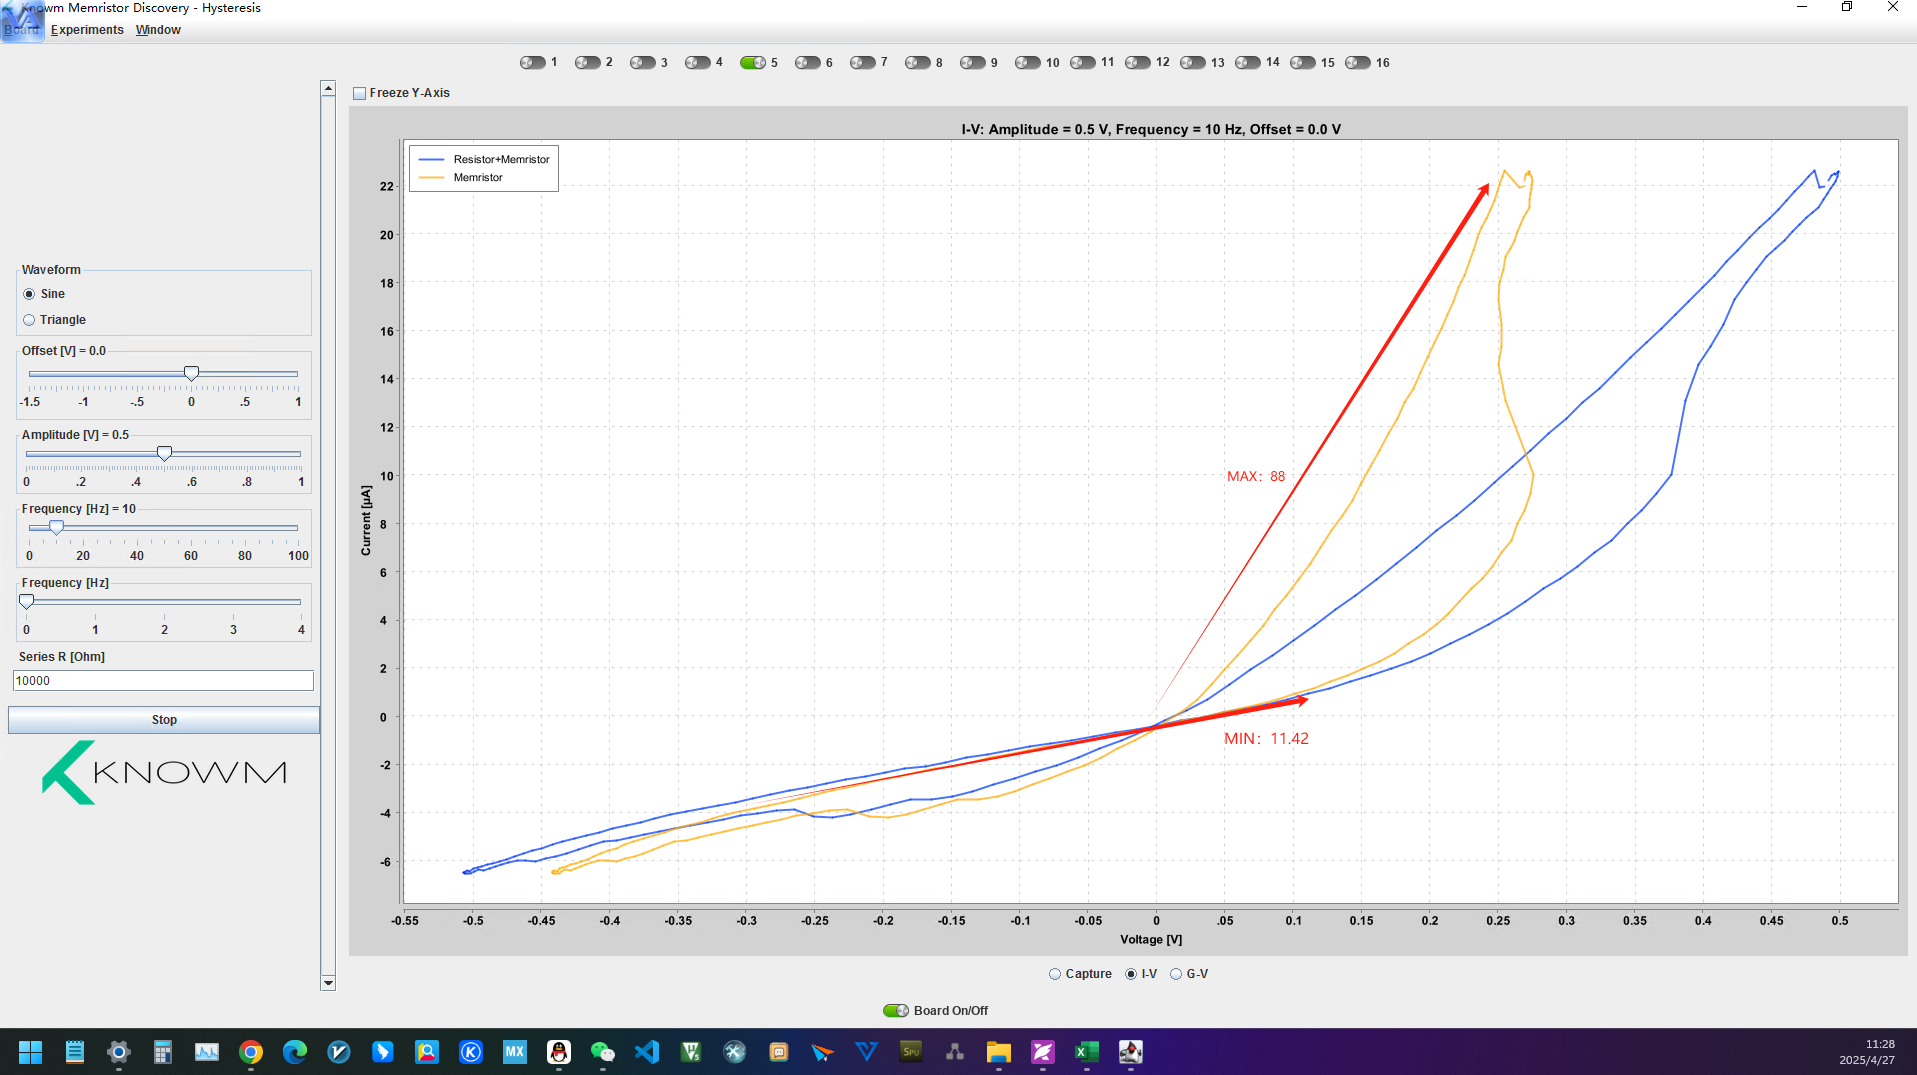
\includegraphics[width=1\textwidth]{figures/F101D.png}
        \caption{F=10,斜率法测量}
        \label{fig:F10_slope_method}
    \end{minipage}
\end{figure}

\begin{figure}[H]
    \centering
    \begin{minipage}{1\textwidth}
        \centering
        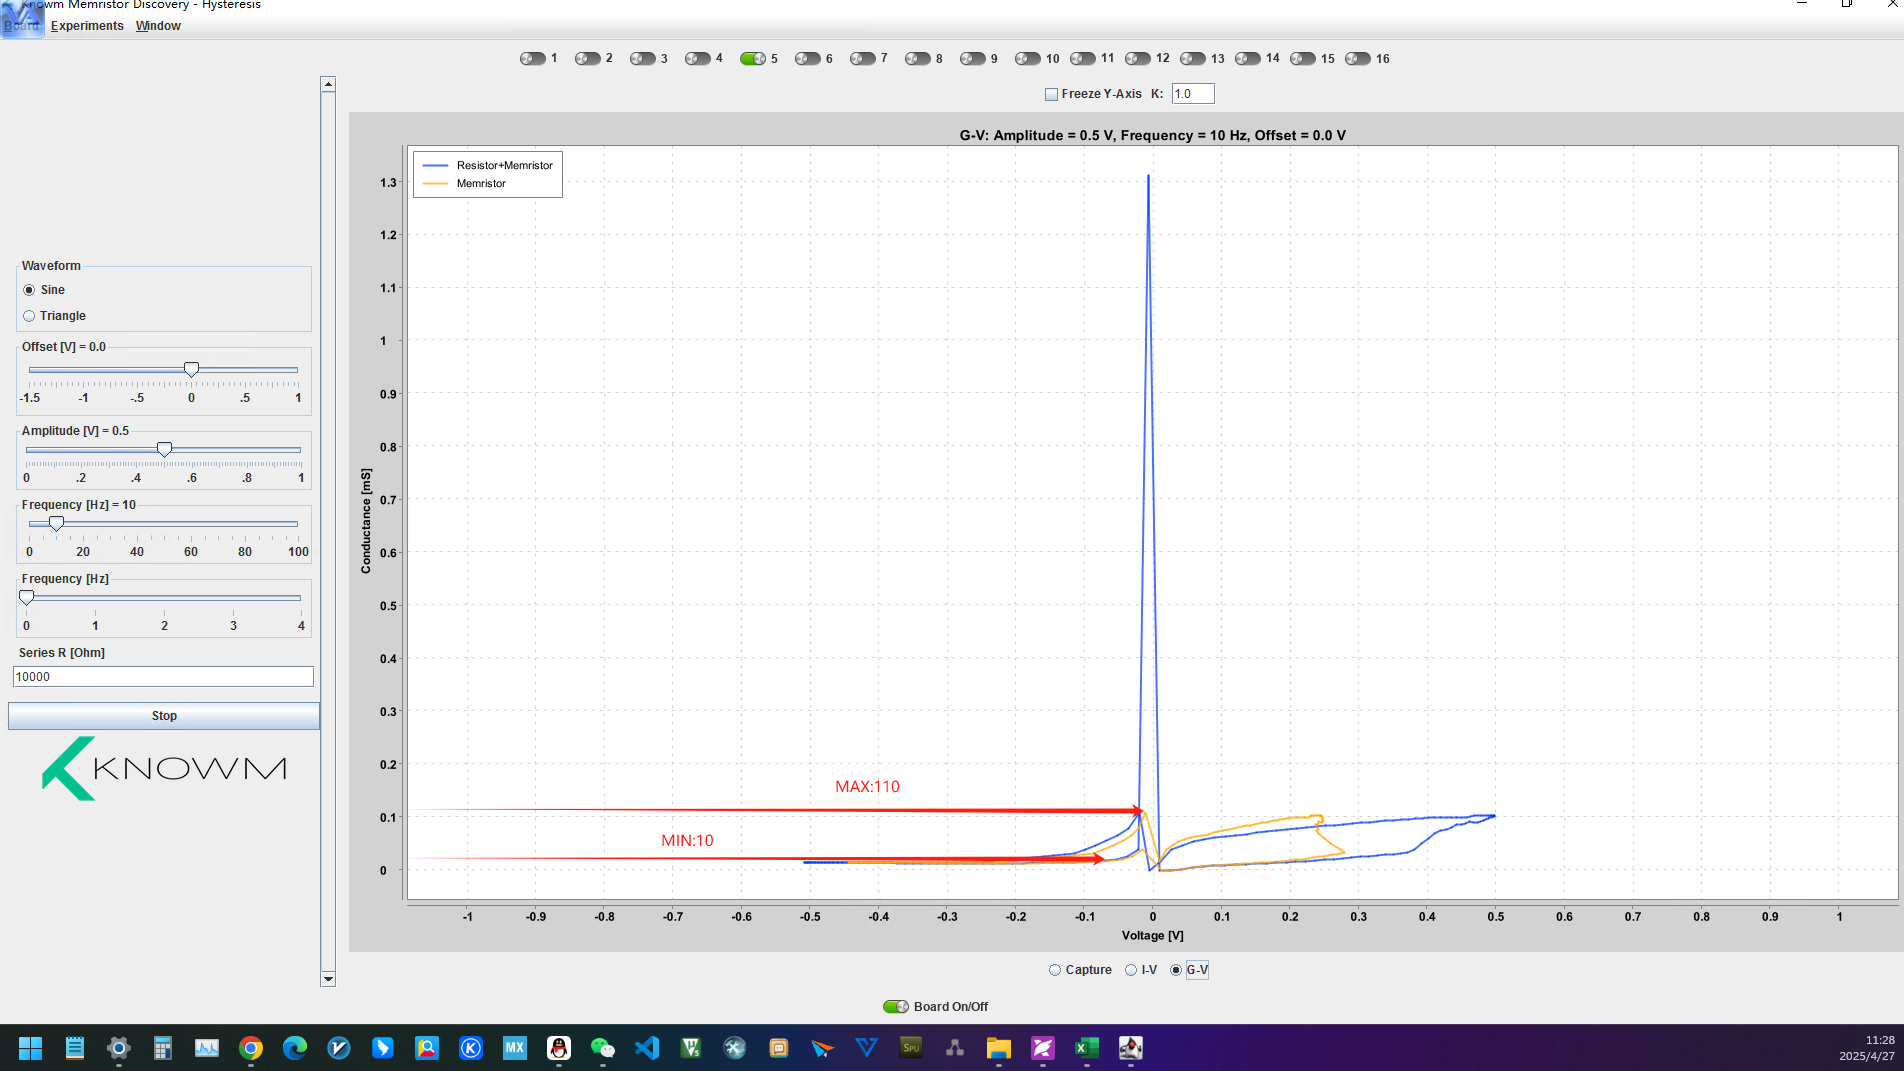
\includegraphics[width=1\textwidth]{figures/F102D.png}
        \caption{F=10,G-V直接读数法测量}
        \label{fig:F10_GV_method}
    \end{minipage}
\end{figure}

\begin{figure}[H]
    \centering
    \begin{minipage}{1\textwidth}
        \centering
        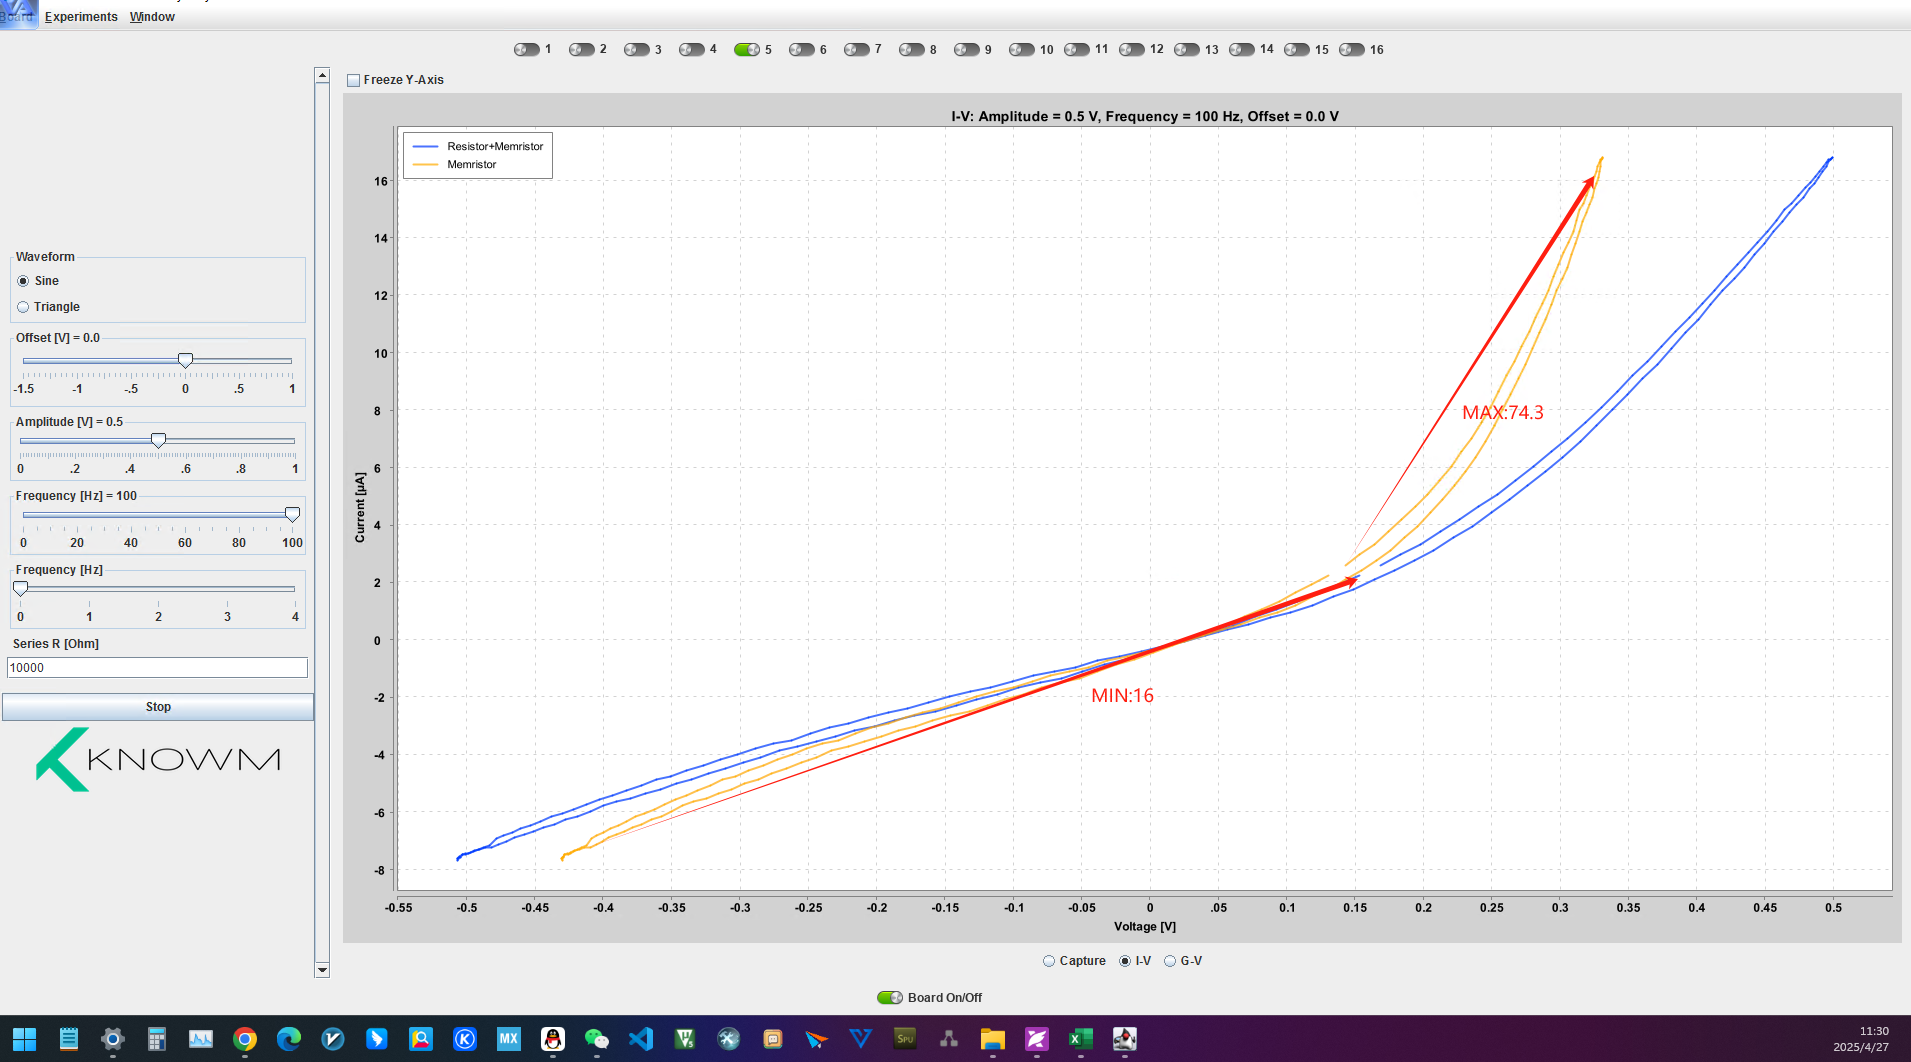
\includegraphics[width=1\textwidth]{figures/F1001D.png}
        \caption{F=100,斜率法测量}
        \label{fig:F100_slope_method}
    \end{minipage}
\end{figure}

\begin{figure}[H]
    \centering
    \begin{minipage}{1\textwidth}
        \centering
        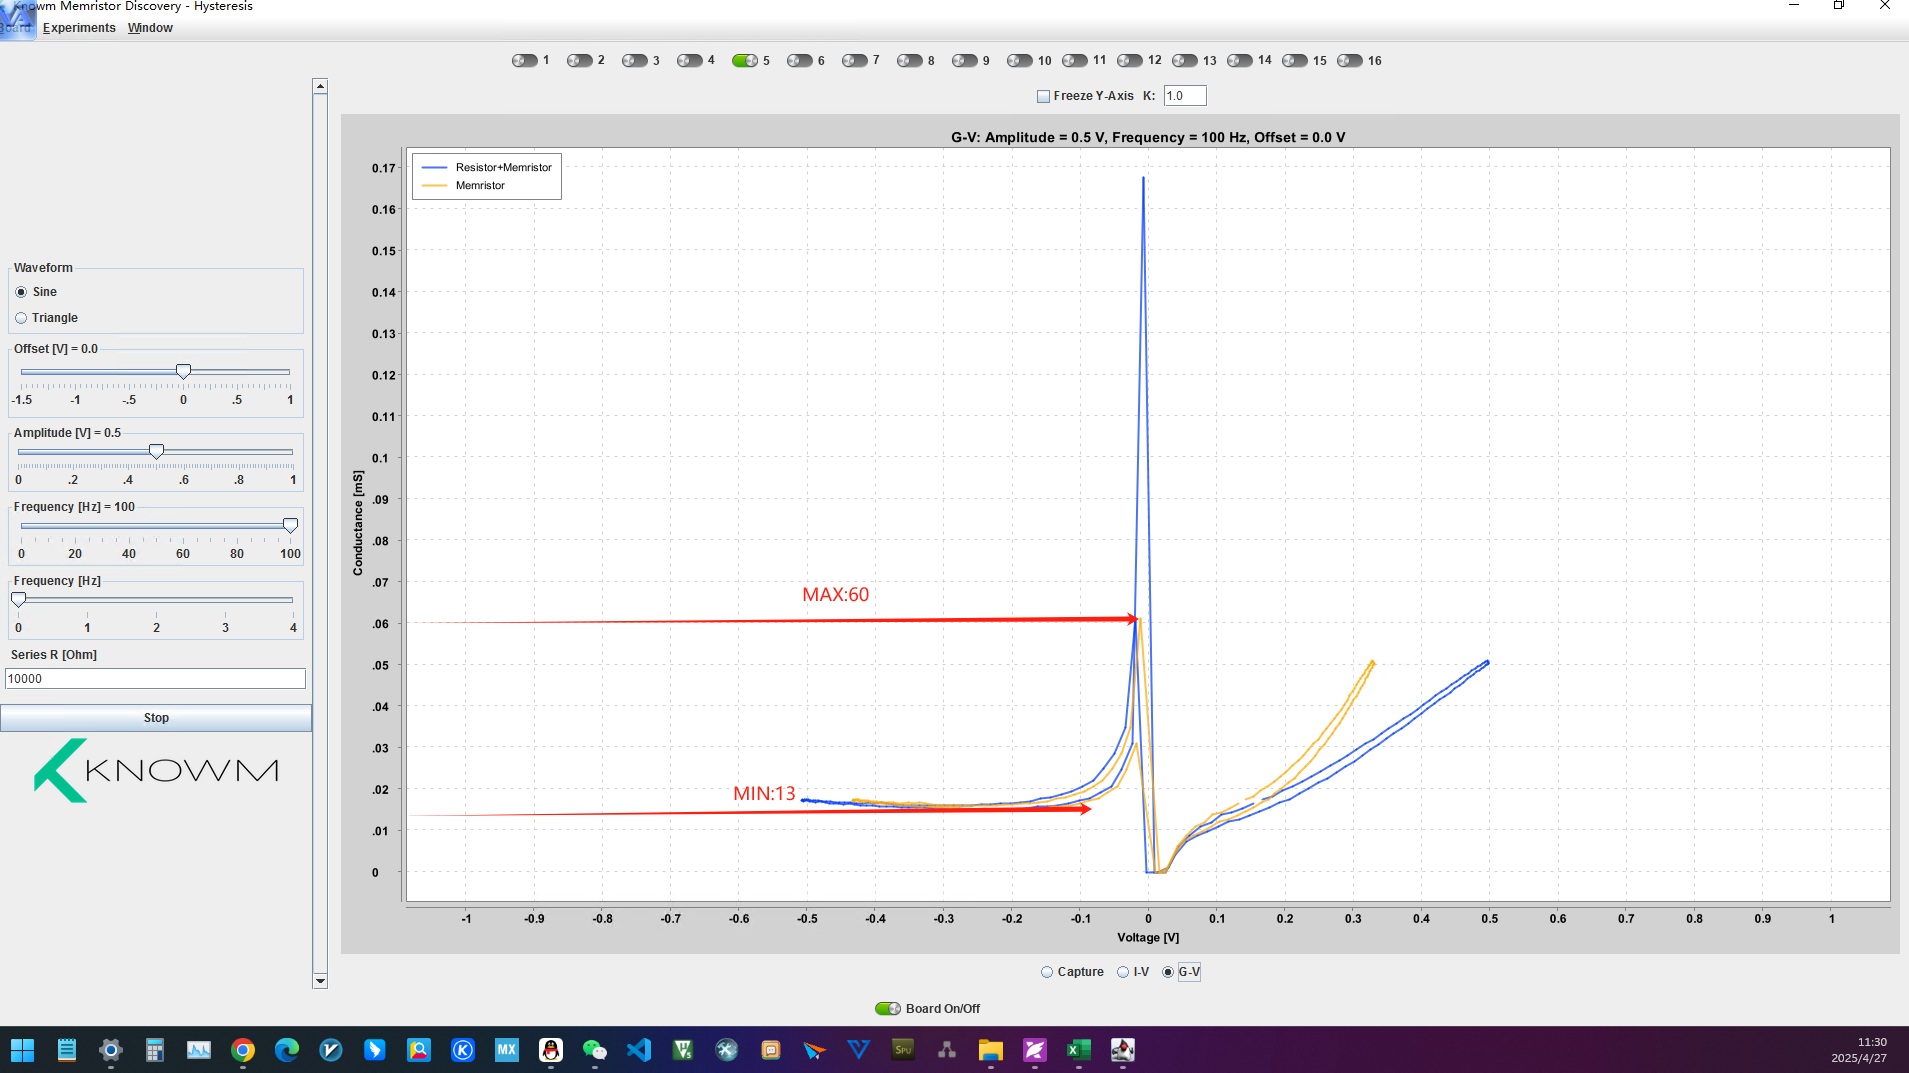
\includegraphics[width=1\textwidth]{figures/F1002D.png}
        \caption{F=100,G-V直接读数法测量}
        \label{fig:F100_GV_method}
    \end{minipage}
\end{figure}

\begin{figure}[H]
    \centering
    \begin{minipage}{1\textwidth}
        \centering
        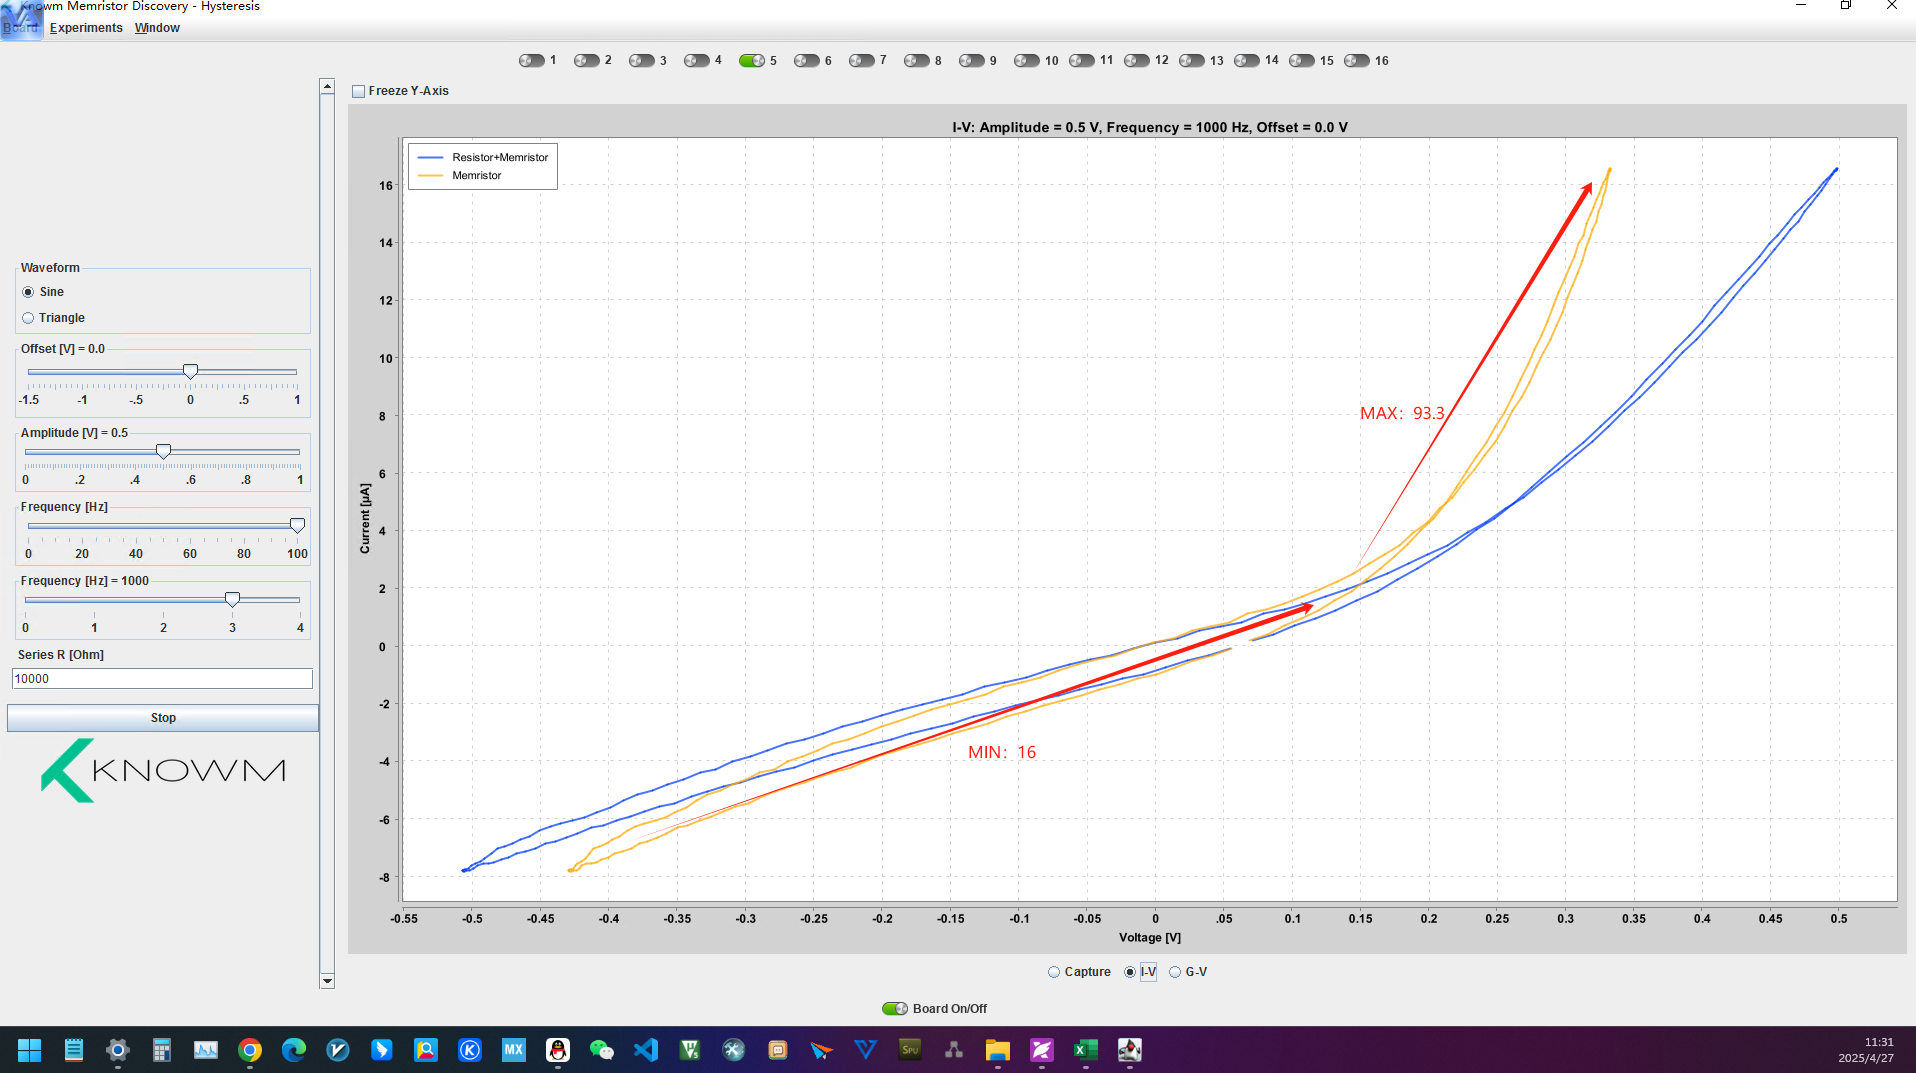
\includegraphics[width=1\textwidth]{figures/F10001D.png}
        \caption{F=1000,斜率法测量}
        \label{fig:F1000_slope_method}
    \end{minipage}
\end{figure}

\begin{figure}[H]
    \centering
    \begin{minipage}{1\textwidth}
        \centering
        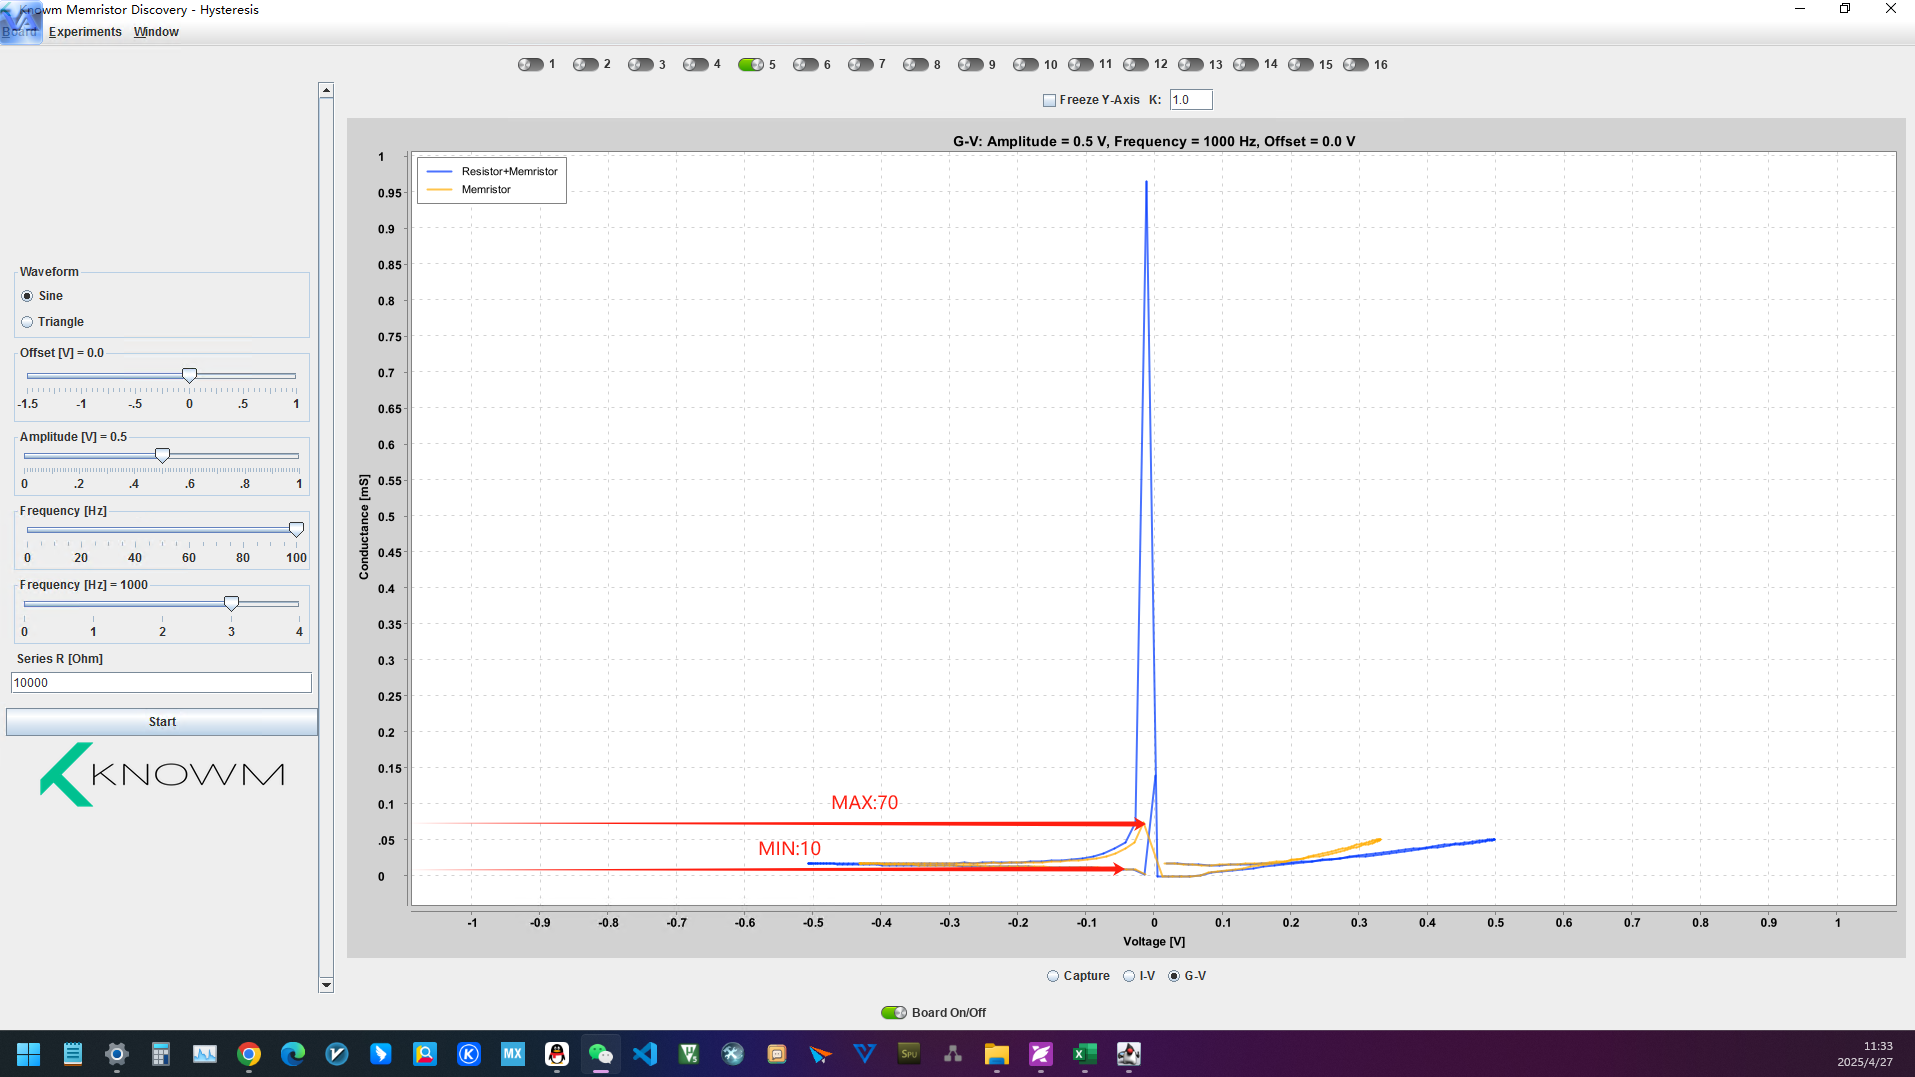
\includegraphics[width=1\textwidth]{figures/F10002D.png}
        \caption{F=1000,G-V直接读数法测量}
        \label{fig:F1000_GV_method}
    \end{minipage}
\end{figure}


\end{document}

